\chapter{Experiments}
\quad \  \ We test the framework with two different application – Bilateral\cite{bilateral} and Local Laplacian\cite{locallaplacian} which are Halide example with tuned schedule for CPU and GPU at three different platform including android platform (Nexus 7) ,detail platform information is shown as table ~\ref{platform1}~\ref{platform2} ,we got at most 57\% improvement with static dispatch and dynamic dispatch compared to best single device. 

\begin{table}[]
\centering
\caption{Test Platform Hardware information}
\label{platform1}
\begin{tabular}{|l|l|l|}
\hline
Platform & CPU & GPU \\ \hline
Android Nexus 7 & \begin{tabular}[c]{@{}l@{}}Quad-core\\ 1.5 GHz Krait\end{tabular} & \begin{tabular}[c]{@{}l@{}}Adreno\\ 320\end{tabular} \\ \hline
PC 1 & \begin{tabular}[c]{@{}l@{}}Intel(R) Core(TM)\\  i5-4590 CPU @ 3.30GHz\end{tabular} & \begin{tabular}[c]{@{}l@{}}ATI Radeon\\ R7 260X\end{tabular} \\ \hline
PC 2 & \begin{tabular}[c]{@{}l@{}}Intel(R) Core(TM)\\  i5-3470 CPU @ 3.20GHz\end{tabular} & \begin{tabular}[c]{@{}l@{}}NVIDIA\\ GTX 750\end{tabular} \\ \hline
\end{tabular}
\end{table}

\begin{table}[]
\centering
\caption{Test Platform software information}
\label{platform2}
\begin{tabular}{|l|l|l|}
\hline
Platform & Compiler & OpenCL Runtime \\ \hline
Android Nexus 7 & \begin{tabular}[c]{@{}l@{}}Android Ndk r10c\\ Halide release\_2015\_06\_03\end{tabular} & Adreno driver for nexus 7 \\ \hline
PC 1 & \begin{tabular}[c]{@{}l@{}}Clang++ 3.6\\ Halide release\_2015\_06\_03\end{tabular} & AMD APP SDK 3.0 Beta \\ \hline
PC 2 & \begin{tabular}[c]{@{}l@{}}Clang++ 3.6\\ Halide release\_2015\_06\_03\end{tabular} & Nvidia driver 337 \\ \hline
\end{tabular}
\end{table}



At the beginning, we have to prove that it is possible we can improve performance by split work into two partitions. So we took Bilateral and Local Laplacian as our benchmark, in each case we gave same input and try to make halide to compute partial output from 10\% to 90\% on CPU and GPU to show the relationship between execution time and workload. 
\begin{figure}[hbtp]
\centering
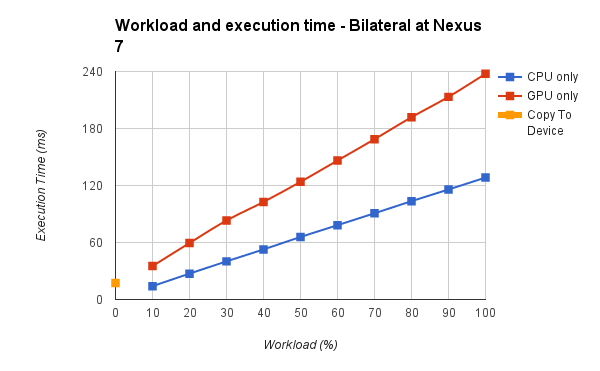
\includegraphics[width=12cm]{img/Result-WorkloadbetweenCPUandGPU(Bilateral@Nexus7).png}
\caption{Result-Bilateral at Nexus 7 }
\label{fig:my_label}
\end{figure}

\begin{figure}[hbtp]
\centering
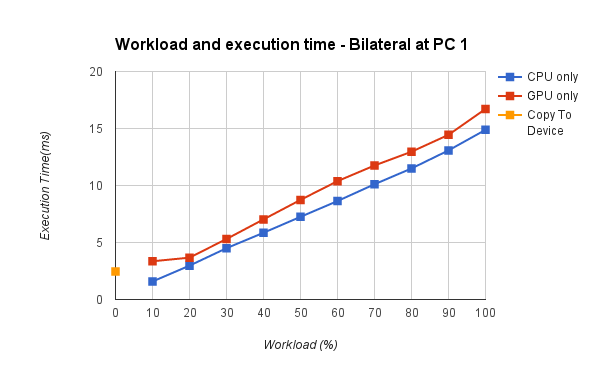
\includegraphics[width=12cm]{img/Result-WorkloadbetweenCPUandGPU(Bilateral@PC1).png}
\caption{Result-Bilateral at PC 1 }
\label{fig:my_label}
\end{figure}

\begin{figure}[hbtp]
\centering
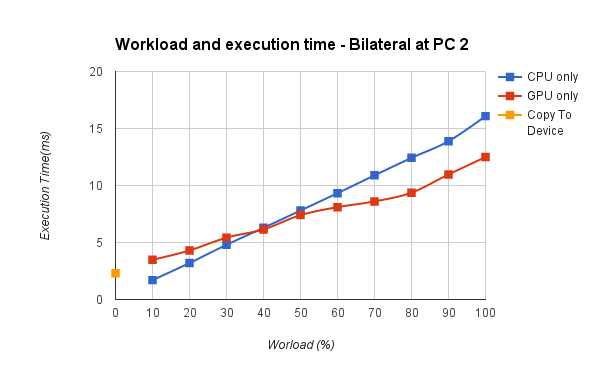
\includegraphics[width=12cm]{img/Result-WorkloadbetweenCPUandGPU(Bilateral@PC2).png}
\caption{Result-Bilateral at PC 2 }
\label{fig:my_label}
\end{figure}

According to experiment result we got, we notice that we could improve performance by split workload into two different devices when processing Bilateral filter. 

%We also test another filter local laplacian the relation between workload and execution time. 
\begin{figure}[hbtp]
\centering
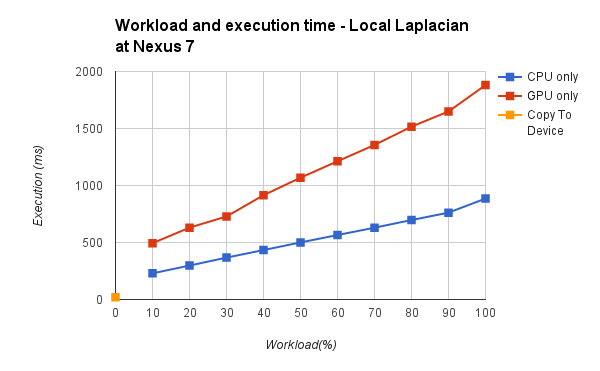
\includegraphics[width=12cm]{img/Result-WorkloadbetweenCPUandGPU(LocalLaplacian@Nexus7).png}
\caption{Result-Loca lLaplacian at Nexus 7 }
\label{fig:my_label}
\end{figure}

\begin{figure}[hbtp]
\centering
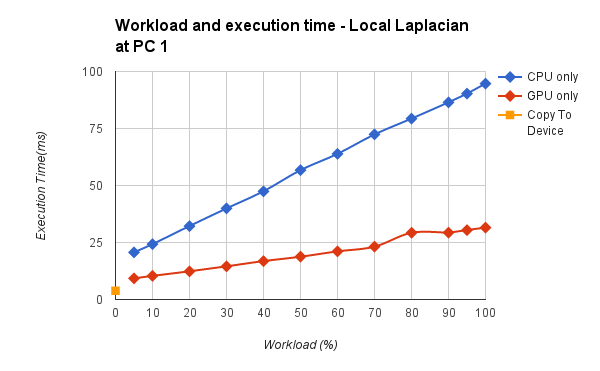
\includegraphics[width=12cm]{img/Result-WorkloadbetweenCPUandGPU(LocalLaplacian@PC1).png}
\caption{Result-Local Laplacian at PC 1 }
\label{fig:my_label}
\end{figure}

\begin{figure}[hbtp]
\centering
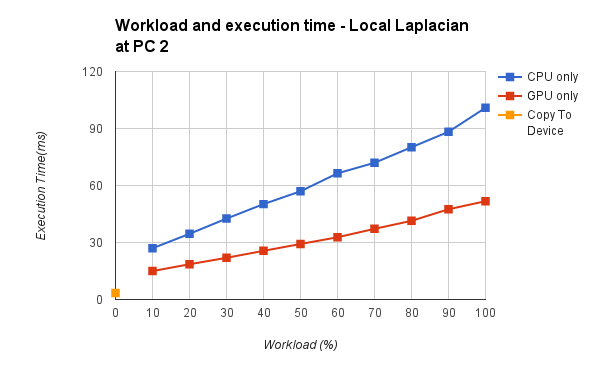
\includegraphics[width=12cm]{img/Result-WorkloadbetweenCPUandGPU(LocalLaplacian@PC2).png}
\caption{Result-Local Laplacian at PC 2 }
\label{fig:my_label}
\end{figure}

We notice that the trend line of Local laplacian is similar to Bilateral. However, there is one little part which is different to Bilateral, that is, according to the trend line, when the workload of bilateral filter equals to zero, the execution time of CPU also equals to zero and the execution time of GPU would equal to the time of copying to device, but the trend line of Local laplacian is not, the trend line of CPU will be higher than zero when the workload equals to zero  and the trend line of GPU will also be higher than the time of coping to device, which means if we split work of local laplacian into 2 or more partition the execution of two or more partition will greater than only 1 partition and it will increase when we split work into more partition, which also implies that we may not get same improvement between static dispatch and dynamic dispatch when the framework handling the case like local laplacian.

\section{Static Dispatch}

\quad \ \ To test static dispatch we assign different workload to CPU and GPU to test the best performance on Static Dispatch. Totally, there are 9 composition between CPU and GPU workload.

In those results, the high peak of the CPU workload and the mapping GPU workload (GPU workload reverse in the diagram) should be the ideal execution time of static dispatch and the line is the real execution time of static dispatch. We got about 1.21x , 1.55x and 1.16x at Nexus7, PC 1 and PC2 respectively when processing bilateral filter compared to best single device. We also got 1.24x, 1.03x and 1.11 speedup improvement at Nexus7, PC 1 and PC2 respectively  when processing Local Laplacian filter compared to best single device. 

However, in the diagrams of Bilateral filter, the static dispatch (the line) is higher than the peak. The gap between high peak and the real static execution time should be overhead of OpenCL runtime, we will profile and discuss the runtime information on next section.

\begin{figure}[hbtp]
\centering
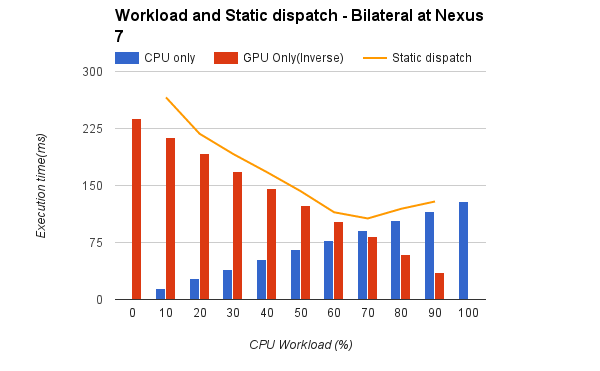
\includegraphics[width=12cm]{img/Result-WorkloadAndStaticDispatch(Bilateral@Nexus7)}
\caption{Result- Bilateral at Nexus 7 }
\label{fig:my_label}
\end{figure}

\begin{figure}[hbtp]
\centering
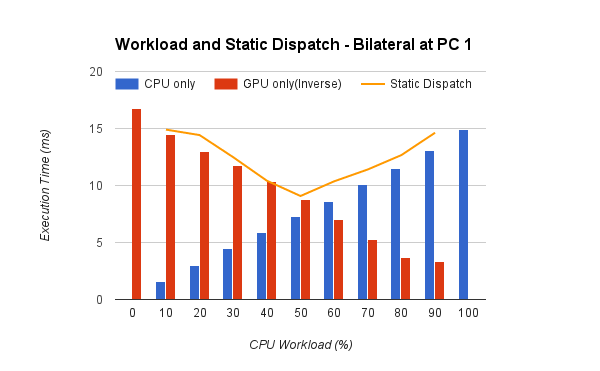
\includegraphics[width=12cm]{img/Result-WorkloadAndStaticDispatch(Bilateral@PC1)}
\caption{Result- Bilateral at PC 1 }
\label{fig:my_label}
\end{figure}

\begin{figure}
\centering
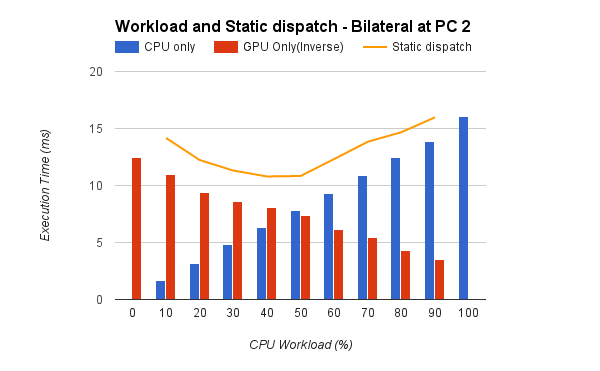
\includegraphics[width=12cm]{img/Result-WorkloadAndStaticDispatch(Bilateral@PC2)}
\caption{Result- Bilateral at PC 2 }
\label{fig:my_label}
\end{figure}


\begin{figure}[hbtp]
\centering
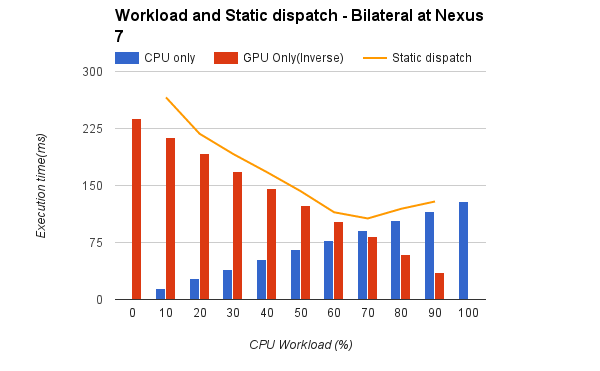
\includegraphics[width=12cm]{img/Result-WorkloadAndStaticDispatch(Bilateral@Nexus7)}
\caption{Result- Local Laplacian at Nexus 7 }
\label{fig:my_label}
\end{figure}

\begin{figure}[hbtp]
\centering
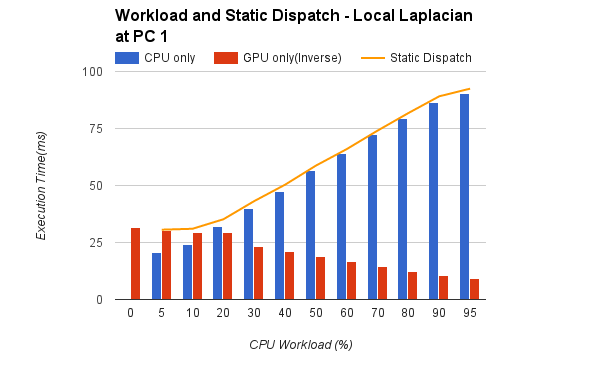
\includegraphics[width=12cm]{img/Result-WorkloadAndStaticDispatch(LocalLaplacian@PC1)}
\caption{Result- Local Laplacian at PC 1}
\label{fig:my_label}
\end{figure}

\begin{figure}[hbtp]
\centering
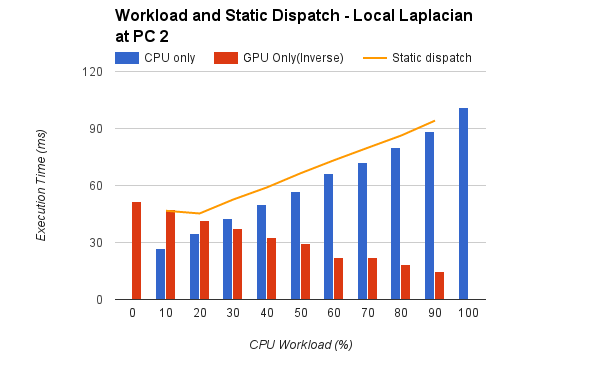
\includegraphics[width=12cm]{img/Result-WorkloadAndStaticDispatch(LocalLaplacian@PC2)}
\caption{Result- Local Laplacian at PC2 }
\label{fig:my_label}
\end{figure}

\section{Dynamic Dispatch}
\quad \  \ After implement static dispatch, we want to implement an easier way to programmer to use both devices, we also implement dynamic dispatch and hope it could be effective as static dispatch.

\begin{figure}[!hbtp]
\centering
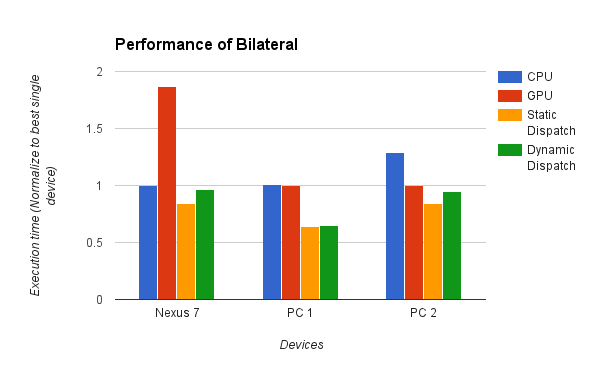
\includegraphics[width=12cm]{img/PerformanceOfBilateral.png}
\caption{Performance of Bilateral filter. For each devices, execution time is shown normalized to the best performing single device – CPU-only or GPU-only.}
\label{fig:my_label}
\end{figure}

\begin{figure}[!hbtp]
\centering
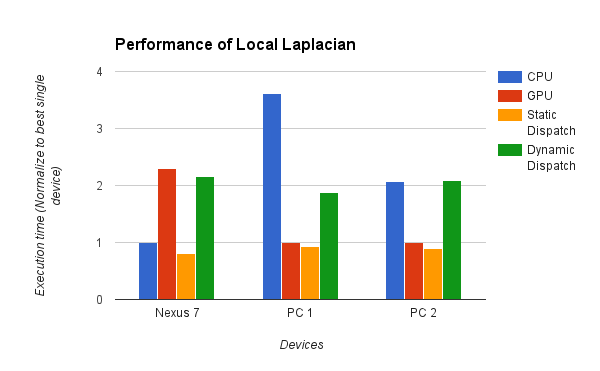
\includegraphics[width=12cm]{img/PerformanceOfLocalLaplacian.png}
\caption{Performance of Local Laplacian  filter. For each devices, execution time is shown normalized to the best performing single device – CPU-only or GPU-only.}
\label{fig:my_label}
\end{figure}

According to the results, it shows that dynamic dispatch will be slower than static dispatch especially when processing filter like local laplacian which matchs our assumption before. It is because filter like local laplacian which will refer to all input data cannot split into multiple blocks or it will refer to all input redundantly. 

\section{Profile OpenCL Runtime information}

\quad \  \ The gap between ideal static execution real static execution should be the overhead of OpenCL runtime information.To prove that, we profile OpenCL runtime information to figure out the bottleneck of our framework. We profile the runtime information of GPU only with processing specific percentage workload and static dispatch with same workload to compare the execution of each stage of OpenCL API.


\begin{figure}[!hbtp]
\centering
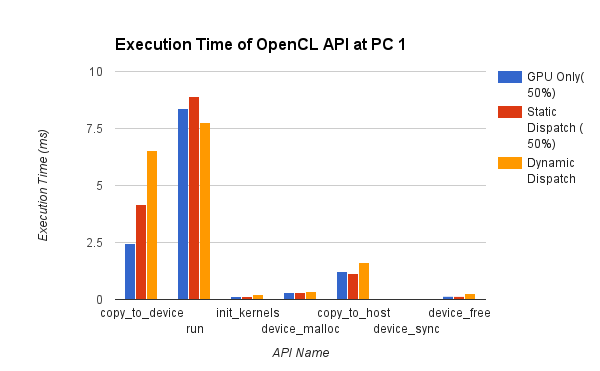
\includegraphics[width=12cm]{img/ExecutionTimeOfAPI(Bilateal@PC1).png}
\caption{Execution time Of OpenCL API at PC1 each API is normalized to GPU only.}
\label{fig:my_label}
\end{figure}

\begin{figure}[!hbtp]
\centering
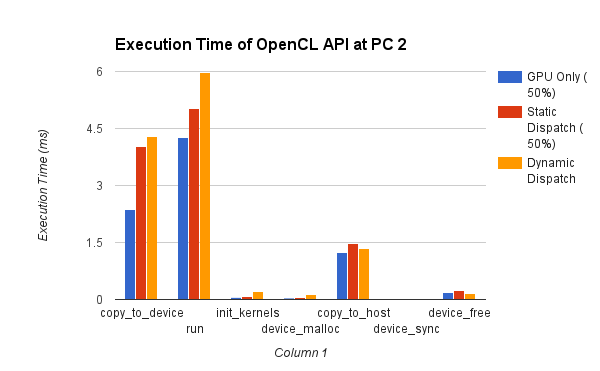
\includegraphics[width=12cm]{img/ExecutionTimeOfAPI(Bilateal@PC2).png}
\caption{Execution time Of OpenCL API at PC2 each API is normalized to GPU only.}
\label{fig:my_label}
\end{figure}

\section{CUDA and OpenCL}
\quad \  \ In addition to OpenCL, Halide also support CUDA as the language of GPU which means our framework should also support CUDA, so we also measured the performance and make a comparison between CUDA and OpenCL when processing bilateral and local laplacian at PC2.



\begin{figure}[hbtp]
\centering
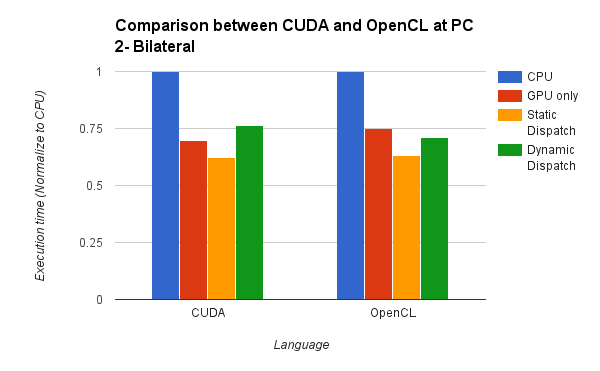
\includegraphics[width=12cm]{img/ComparisonBetweenCUDAAndOpenCL(Bilateral).png}
\caption{Comparison between CUDA and OpenCL when processing Bilateral Filter. Each time is normalized to CPU execution time}
\label{fig:my_label}
\end{figure}

\begin{figure}[hbtp]
\centering
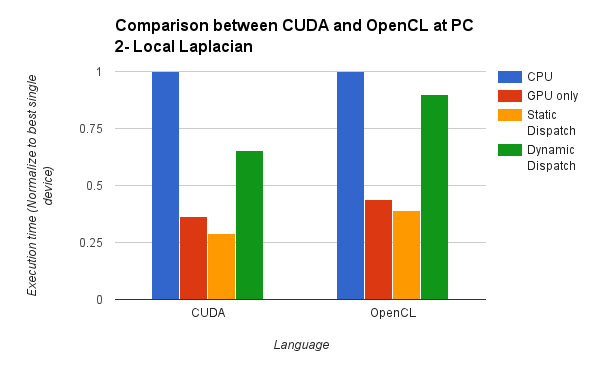
\includegraphics[width=12cm]{img/ComparisonBetweenCUDAAndOpenCL(LocalLaplacian).png}
\caption{Comparison between CUDA and OpenCL when processing Local Laplacian Filter. Each time is normalized to CPU execution time}
\label{fig:my_label}
\end{figure}

\section{Different Input Size}
\quad \  \ To test the influence of different input size, we also experiment different input with 8192*6960 pixel.According to our results, PC 1 can similar to our predict execution time, however, PC 2 still slower to our predict execution time even if we enlarge input size .To figure out the reason, we also profile the API time of this input size, in next section, we will discuss the results.

\begin{figure}[!hbtp]
\centering
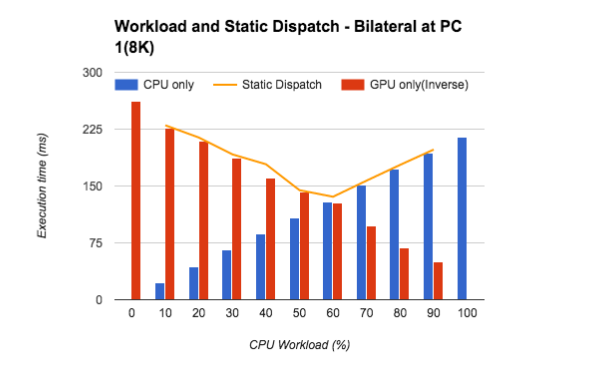
\includegraphics[width=12cm]{img/WorkloadAndStaiticDispatch-BilateralAtPC1(8K).png}
\caption{Result- Bilateral at PC 1 with 8K input size}
\label{fig:my_label}
\end{figure}

\begin{figure}[!hbtp]
\centering
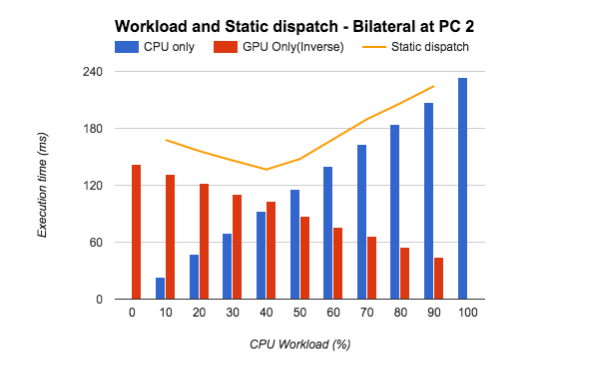
\includegraphics[width=12cm]{img/WorkloadAndStaiticDispatch-BilateralAtPC2(8K).png}
\caption{Result- Bilateral at PC 2 with 8K input size}
\label{fig:my_label}
\end{figure}


\section{OpenCL API exection time with larger size}
\quad \  \ After profiling OpenCL API execution time, Figure ~\ref{fig:ExeTime8KPC2} shows that the gap between GPU only and static dispatch still exists in PC 2 when input size became to 8192*6960.

\begin{figure}[!hbtp]
\centering
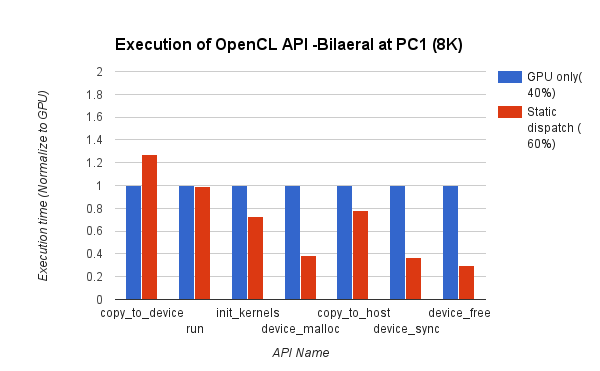
\includegraphics[width=12cm]{img/ExecutionofOpenCLAPI-BilateralatPC1(8K).png}
\caption{Execution time of openCL API - Bilateral at PC 1 (8K)}
\label{fig:ExeTime8KPC1}
\end{figure}

\begin{figure}[!hbtp]
\centering
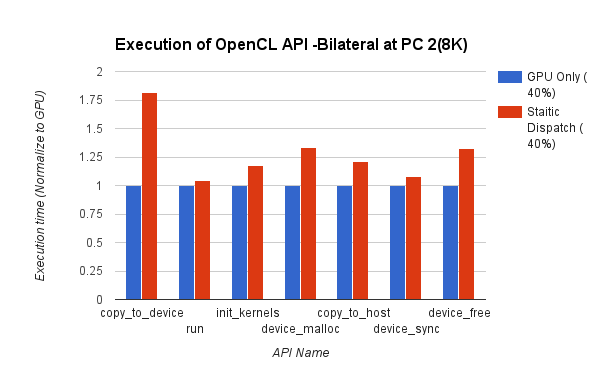
\includegraphics[width=12cm]{img/ExecutionofOpenCLAPI-BilateralatPC2(8K).png}
\caption{Execution time of openCL API - Bilateral at PC 2 (8K)}
\label{fig:ExeTime8KPC2}
\end{figure}



